\documentclass{scrartcl}

\usepackage[utf8]{inputenc}
\usepackage[english, ngerman]{babel}
\usepackage[autostyle]{csquotes}
\usepackage{caption}
\usepackage[hidelinks]{hyperref}
\usepackage{enumerate}
\usepackage{graphicx}
\usepackage{pdfpages}

%\title{Hashtag Inspektor (Android)}
%\subtitle{Group: HashtagInspectors}
%\author{
%Mohammad Sajjad Khoshrou: \url{khoshrou@uni-bremen.de}
%\and Thanh Nguyen Chi: \url{nguyenct@uni-bremen.de}
%\and Simon Glaser: \url{sglaser@uni-bremen.de}
%\and Vinzenz Tecker: \url{vtecker@uni-bremen.de }
%}

\pagenumbering{gobble}

\begin{document}
%\maketitle
\begin{center}
\sffamily
\huge{\textbf {Hashtag Inspektor (Android)}}\\
\vspace{5pt}
\large{\textbf{Gruppe: Hashtag Inspectors}}\\
\vspace{10pt}
\rmfamily
Mohammad Sajjad Khoshrou: \url{khoshrou@uni-bremen.de} \\
Thanh Nguyen Chi: \url{nguyenct@uni-bremen.de} \\
Simon Glaser: \url{sglaser@uni-bremen.de} \\
Vinzenz Tecker: \url{vtecker@uni-bremen.de} \\
\end{center}

\section*{Beschreibung}
Wir möchten eine App mit AndroidStudio erstellen, mit der man nach Hashtags (\#) auf Twitter suchen und alle mit dem gesuchten \# in Verbindung stehenden Tags finden kann. Die App soll dem Nutzer dabei helfen, Twitter-Trends zu analysieren indem er \#'s finden kann, die häufig benutzt werden. 
Sucht man z.B. nach \enquote{\#Apfelbaum}, so listet die App alle \#'s auf, die zusätzlich zu \enquote{\#Apfelbaum} erwähnt werden und sortiert das Ergebnis nach Häufigkeit. \\
Die resultierende Liste könnte beispielsweise so aussehen:
\begin{quotation}
Suche nach: \enquote{\#Apfelbaum}
\begin{enumerate}
\item \enquote{\#Obst} 60x erwähnt
\item \enquote{\#Essen} 35x erwähnt
\item \enquote{\#Gesund} 12x erwähnt
\end{enumerate}
100 Tweets wurden durchsucht.
\end{quotation}
Die Suche kann allgemein, ohne bestimmte Parameter stattfinden, oder wir schränken die Suche auf einen bestimmten Ort oder ein bestimmtes Land ein. Diese Anforderungen lassen sich alle mithilfe der Search API von Twitter durchführen. Da die App sich mit Trends beschäftigt, wird es auch eine Funktion geben, mit der man die \#-Trends eines bestimmten Ortes oder Landes einsehen kann um diese \# zu analysieren.\\
Falls machbar, soll es die App außerdem ermöglichen, die Stimmung der Tweets mit dem gesuchten \# einzuschätzen. Die Analyse könnte dann mithilfe eines Tools wie zum Beispiel Google Natural Language\footnote{\url{https://cloud.google.com/natural-language/}} oder der Sentiment Analysis API\footnote{\url{http://text-processing.com/docs/sentiment.html}} erfolgen. Beim \enquote{\#Apfelbaum} Beispiel könnte das Ergebnis der Analyse folgendermaßen aussehen:
%\begin{quotation}
% Tweets für \#Apfelbaum:\\
%35 \% positiv, 5 \% negativ, 60\% neutral
\begin{figure}[h]
\centering
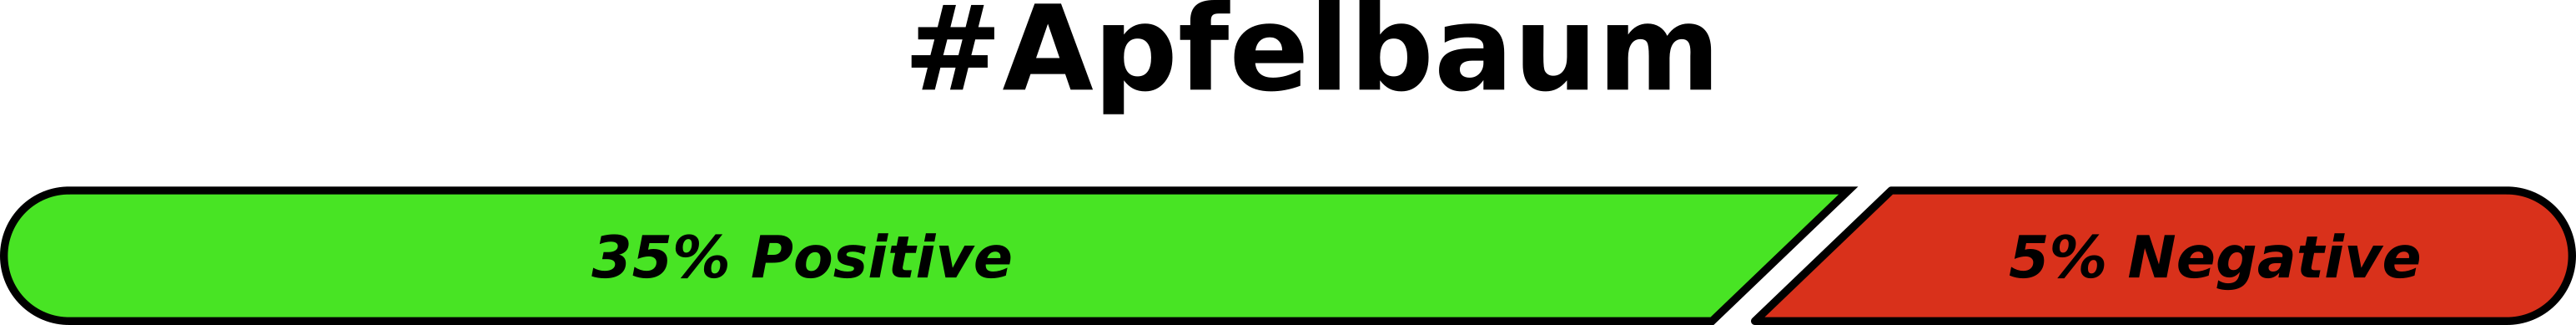
\includegraphics[width=.5\textwidth]{sentimentVisualize.png}
\caption*{35 \% positive Tweets für \enquote{\#Apfelbaum}, 5 \% negativ. Der Rest ist neutral oder nicht auswertbar.}
\end{figure}
%\end{quotation}

\newpage
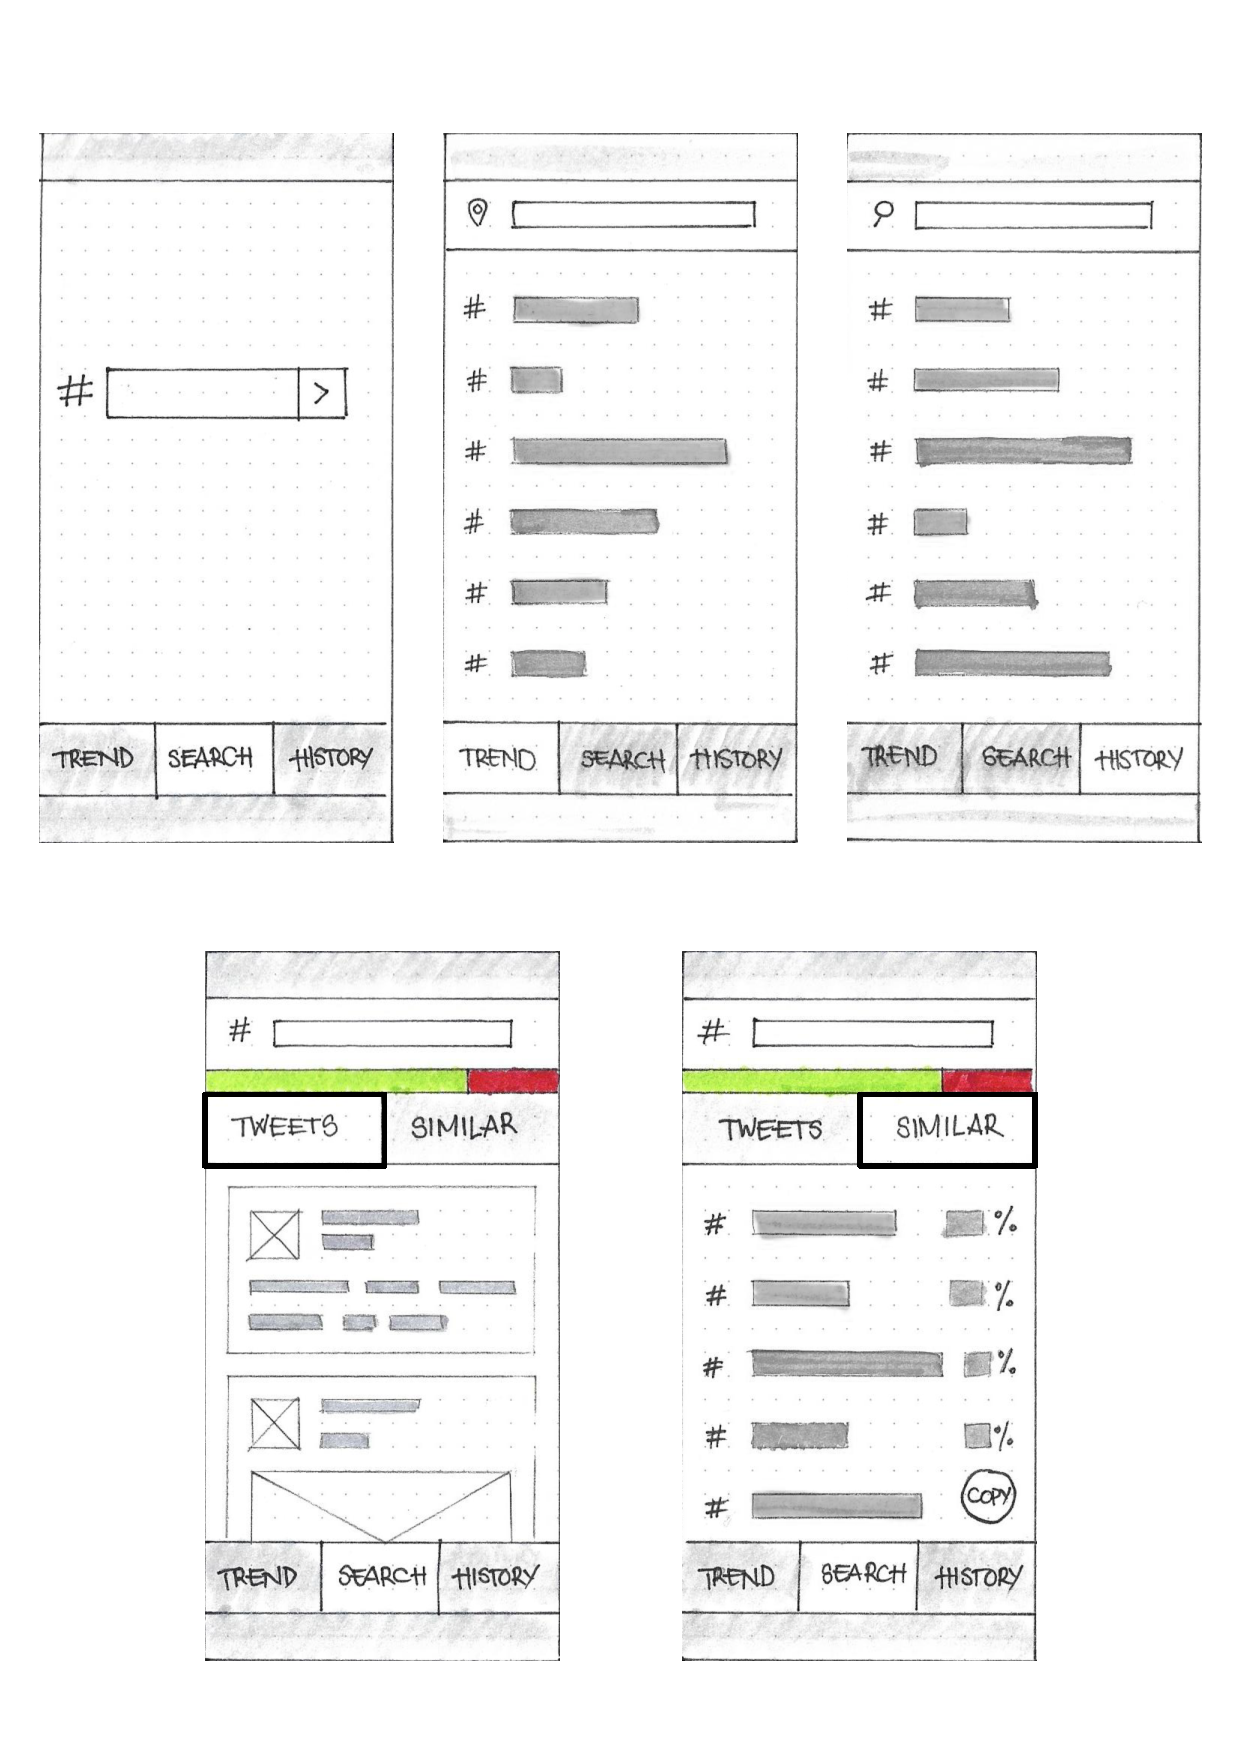
\includepdf[pages=-]{Prototyp.pdf}
\newpage
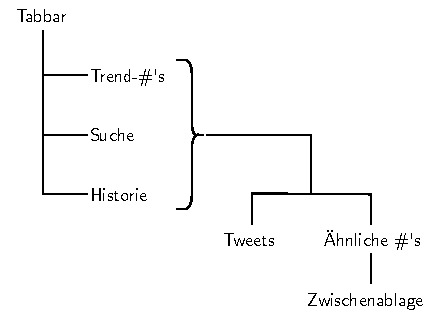
\includepdf[pages=-]{Navigationsbaum.pdf}
\end{document}